\section{Condutores, infraestrutura e queda de tensão}

\begin{frame}{Dimensionamento: não existe um único critério}
\small
\begin{columns}[T,onlytextwidth]
\column{0.52\textwidth}
\begin{caixaNorma}[title=Fluxo de decisão]
A seção final deve atender simultaneamente a:
\begin{itemize}
\item seção mínima;
\item capacidade de condução de corrente;
\item queda de tensão;
\item curto-circuito/estabilidade térmica;
\item proteção contra choque/desligamento automático;
\item requisitos mecânicos e de instalação.
\end{itemize}
\end{caixaNorma}
\column{0.46\textwidth}
\centering
\begin{tikzpicture}[node distance=0.25cm,every node/.style={font=\scriptsize}]
\tikzset{b/.style={draw=corPrim,fill=corDef!7,rounded corners,align=center,minimum width=3.6cm,minimum height=0.58cm}}
\node[b] (a) {$I_b$ e regime};
\node[b,below=of a] (b) {Método de instalação};
\node[b,below=of b] (c) {Fatores de correção};
\node[b,below=of c] (d) {$I_b\le I_n\le I_z$};
\node[b,below=of d] (e) {Queda de tensão};
\node[b,below=of e] (f) {Curto + PE + desligamento};
\foreach \u/\v in {a/b,b/c,c/d,d/e,e/f}{\draw[-{Stealth},thick,corPrim] (\u)--(\v);}
\end{tikzpicture}
\end{columns}
\end{frame}

\begin{frame}{Coordenação carga--proteção--condutor}
\small
\begin{columns}[T,onlytextwidth]
\column{0.51\textwidth}
\begin{align*}
I_b &\le I_n \le I_z\\
I_2 &\le 1{,}45 I_z
\end{align*}
\begin{itemize}
\item $I_b$: corrente de projeto.
\item $I_n$: corrente nominal/ajuste do dispositivo.
\item $I_z$: capacidade do condutor após correções.
\item $I_2$: corrente convencional de atuação para sobrecarga.
\end{itemize}
\column{0.47\textwidth}
\centering
\begin{tikzpicture}[scale=0.9,every node/.style={font=\scriptsize}]
\draw[->] (0,0)--(5,0) node[right]{$I$};
\draw[thick,corDef] (1.0,0.1)--(1.0,1.1) node[above]{$I_b$};
\draw[thick,corAccent] (2.0,0.1)--(2.0,1.6) node[above]{$I_n$};
\draw[thick,corNorma] (3.3,0.1)--(3.3,1.2) node[above]{$I_z$};
\draw[decorate,decoration={brace,amplitude=5pt}] (1,-0.25)--(3.3,-0.25) node[midway,below=5pt]{coordenação};
\end{tikzpicture}
\end{columns}
\end{frame}

\begin{frame}{Fatores de correção térmica}
\small
\begin{tabularx}{\textwidth}{>{\bfseries}p{3.2cm}X}
\toprule
Fator & Consequência \\
\midrule
Temperatura ambiente & Aumenta temperatura de operação e reduz capacidade admissível. \\
Agrupamento & Circuitos próximos aquecem mutuamente. \\
Isolação térmica & Pode impedir dissipação e exigir forte redução de corrente. \\
Método de instalação & Eletroduto, leito, bandeja, enterrado e ao ar têm comportamentos diferentes. \\
Tipo de isolação & PVC, EPR/XLPE etc. possuem limites térmicos distintos. \\
Harmônicas & Aumentam perdas e podem elevar corrente no neutro. \\
\bottomrule
\end{tabularx}
\vspace{2mm}
\begin{caixaAt}
A corrente de catálogo do cabo não pode ser copiada sem identificar o método de referência e os fatores aplicáveis.
\end{caixaAt}
\end{frame}

\begin{frame}{Neutro em presença de harmônicas triplas}
\small
\begin{columns}[T,onlytextwidth]
\column{0.50\textwidth}
\begin{itemize}
\item Em sistema equilibrado senoidal, a fundamental do neutro tende a se cancelar.
\item Componentes de ordem 3, 9, 15... são de sequência zero e podem \textbf{somar} no neutro.
\item Fontes chaveadas monofásicas em grande quantidade exigem atenção especial.
\end{itemize}
\begin{caixaAt}
Não reduzir o neutro automaticamente em escritórios, data centers, laboratórios ou instalações com muita eletrônica.
\end{caixaAt}
\column{0.48\textwidth}
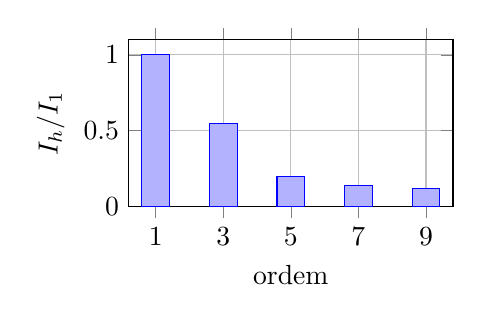
\begin{tikzpicture}
\begin{axis}[width=5.7cm,height=3.7cm,ybar,bar width=10pt,xlabel={ordem},ylabel={$I_h/I_1$},ymin=0,ymax=1.1,xtick={1,3,5,7,9},grid=major]
\addplot coordinates {(1,1)(3,0.55)(5,0.20)(7,0.14)(9,0.12)};
\end{axis}
\end{tikzpicture}
\end{columns}
\end{frame}

\begin{frame}[shrink=5]{Queda de tensão}
\small
\begin{columns}[T,onlytextwidth]
\column{0.53\textwidth}
\begin{align*}
\Delta V_{1\phi}&\approx2IL(R'\cos\varphi+X'\sen\varphi)\\
\Delta V_{3\phi}&\approx\sqrt3IL(R'\cos\varphi+X'\sen\varphi)\\
\Delta V(\%)&=100\frac{\Delta V}{V_n}
\end{align*}
\begin{itemize}
\item $L$ é o comprimento de ida; $R'$ e $X'$ são valores por unidade de comprimento, na condição de operação considerada. Usar unidades compatíveis, por exemplo km com $\Omega$/km.
\item Em $1\phi$, o fator 2 já representa ida e retorno; não duplicar novamente o comprimento.
\item Usar $V_n=V_{FN}$ no circuito monofásico e $V_n=V_{LL}$ no trifásico.
\item Circuitos longos podem ser dimensionados pela queda, não pela ampacidade.
\end{itemize}
\column{0.45\textwidth}
\begin{caixaEx}
Trifásico: $I=\SI{40}{A}$, $L=\SI{80}{m}$, $R'=\SI{3.08}{\ohm/km}$, $X'=\SI{0.08}{\ohm/km}$, $fp=0{,}85$.
\[
\Delta V\approx\SI{14.7}{V}\Rightarrow 3{,}9\%\;@\;\SI{380}{V}.
\]
A aceitação depende do limite aplicável ao trecho e ao sistema completo.
\end{caixaEx}
\end{columns}
\end{frame}

\begin{frame}{Efeito do comprimento: corrente de falta e queda}
\small
\centering
\begin{tikzpicture}
\begin{axis}[width=10.8cm,height=4.6cm,xlabel={distância ao quadro/fonte (m)},ylabel={valor normalizado},xmin=0,xmax=250,ymin=0,ymax=1.1,grid=both,legend pos=north east]
\addplot[corPrim,thick,smooth] coordinates {(0,1)(25,0.82)(50,0.67)(75,0.56)(100,0.47)(150,0.36)(200,0.29)(250,0.24)};
\addlegendentry{$I_{cc}$ relativo}
\addplot[corAccent,thick,dashed,smooth] coordinates {(0,0)(25,0.10)(50,0.20)(75,0.30)(100,0.40)(150,0.60)(200,0.80)(250,1.00)};
\addlegendentry{$\Delta V$ relativo}
\end{axis}
\end{tikzpicture}
\begin{caixaObs}
Quanto mais distante: maior queda de tensão e, em geral, menor corrente de curto. Isso pode alterar seção e tempo de desligamento.
\end{caixaObs}
\end{frame}

\begin{frame}{Curto-circuito: verificação térmica do condutor}
\small
\begin{columns}[T,onlytextwidth]
\column{0.51\textwidth}
\begin{align*}
S &\ge \frac{I_k\sqrt{t}}{k}
\end{align*}
\begin{itemize}
\item $S$: seção do condutor.
\item $I_k$: corrente de falta considerada.
\item $t$: duração até eliminação.
\item $k$: constante relacionada ao material e isolação.
\end{itemize}
\column{0.47\textwidth}
\begin{caixaEx}
Se um PE conduz $\SI{4}{kA}$ por $\SI{0.2}{s}$ e o valor adotado para $k$ for $115$:
\[
S\ge\frac{4000\sqrt{0{,}2}}{115}\approx\SI{15.6}{mm^2}.
\]
Escolhe-se seção comercial e verifica-se o conjunto de critérios.
\end{caixaEx}
\end{columns}
\end{frame}

\begin{frame}{Condutor de proteção: seção também é calculada}
\small
\begin{columns}[T,onlytextwidth]
\column{0.50\textwidth}
\begin{caixaNorma}[title=Método tabular simplificado]
Para condutores de fase e PE do mesmo material e nas condições previstas pelo método:
\[
S_{PE}=\begin{cases}
S_F, & S_F\le\SI{16}{mm^2}\\
\SI{16}{mm^2}, & \SI{16}{mm^2}<S_F\le\SI{35}{mm^2}\\
S_F/2, & S_F>\SI{35}{mm^2}
\end{cases}
\]
\end{caixaNorma}
\column{0.48\textwidth}
\begin{caixaAt}[title=O que ainda precisa fechar]
\begin{itemize}
\item seção mínima e proteção mecânica;
\item condição adiabática $S\ge I_k\sqrt{t}/k$;
\item impedância do caminho de falta e tempo de desligamento;
\item conexões, continuidade e identificação;
\item requisitos específicos de equipotencialização.
\end{itemize}
\end{caixaAt}
\end{columns}
\end{frame}

\begin{frame}{Eletrodutos, bandejas e segregação}
\small
\begin{columns}[T,onlytextwidth]
\column{0.50\textwidth}
\begin{itemize}
\item Ocupação deve permitir lançamento e substituição de cabos.
\item Respeitar raios de curvatura e esforços de tração.
\item Separar potência, controle, instrumentação e dados conforme compatibilidade e isolamento.
\item Considerar expansão e acessibilidade.
\item Bandejas metálicas precisam integrar o conceito de equipotencialização quando aplicável.
\end{itemize}
\column{0.48\textwidth}
\centering
\begin{tikzpicture}[scale=0.78]
\draw[thick,corPrim] (0,0) rectangle (5.8,2.1);
\foreach \x in {0.25,0.65,...,5.55}{\draw[black!25] (\x,0)--(\x,2.1);}
\foreach \x/\y/\c in {0.7/1.45/corPrim,1.5/0.7/corAccent,2.5/1.3/corAt,3.4/0.55/corNorma,4.3/1.5/corDef,5.1/0.85/corPrim}{\fill[\c!70] (\x,\y) circle (0.18);\draw (\x,\y) circle (0.18);}
\node at (2.9,-0.45) {leito/bandeja: rota também é parte do projeto};
\end{tikzpicture}
\end{columns}
\end{frame}

\begin{frame}{Identificação de condutores e circuitos}
\small
\begin{columns}[T,onlytextwidth]
\column{0.50\textwidth}
\begin{tabularx}{\textwidth}{>{\bfseries}p{2.1cm}X}
\toprule
Elemento & Princípio \\
\midrule
PE & Identificação exclusiva de proteção. \\
Neutro & Identificação própria e coerente. \\
Fases & Padrão consistente em toda a instalação. \\
Retornos & Anilhas/etiquetas; não confundir com PE/N. \\
Cabos & Origem, destino, circuito e seção. \\
\bottomrule
\end{tabularx}
\column{0.48\textwidth}
\begin{caixaProjeto}[title=As built útil]
Registrar:
\begin{itemize}
\item identificação real;
\item bornes e dispositivos;
\item ajustes de proteção;
\item cabos instalados;
\item alterações de campo;
\item reservas e circuitos desativados.
\end{itemize}
\end{caixaProjeto}
\end{columns}
\end{frame}

%=====================================================================
